\chapter{Experiment Design}\label{sec-DOE}
This chapter talks about the Experiment set up.
\section{ArduSat}
The HKUST CYT Lab has a lot of ArduSat DemosSat. ArduSat is an Arduino based Nanosatellite, based on the CubeSat standard. It contains a set of Arduino boards and sensors. The general public will be allowed to use these Arduinos and sensors for their own creative purposes while they are in space. 
\begin{figure}
\centering
\includegraphics[width=6cm]{fig/DOE/Demosat}
\caption{ArduSat DemoSat}
\end{figure}
The DemoSat is designed to the CubeSat One Unit (1U) standard. The 3D printed frame comes fully assembled with standoffs and see-through acrylic platforms. Each DemoSat also includes all of the components included in the Because Learning Sensor Kit. The Because Learning Sensor Kit includes:
\begin{enumerate}
\item Microcontroller programmed w/ Arduino 
\item Because Learning 'Sensor board' sensors 
\begin{itemize}
\item Accelerometer
\item Gyroscope
\item Magnetometer
\end{itemize}
\end{enumerate} 
Also the DemoSat includes two wireless radio frequency (RF) radios. They are Digi XBee 2.4Ghz modules. One is connected inside the DemoSat and the second is connect via USB to labptop. By doing this it enables the DemoSatellite to communicate up to 1500 meter from the computer.
It can get our interested acceleration, angular rate and orientation of the Satellites at real time wirelessly.
\subsection{Arduino Data Acquisition}
Our interested physical quantities are acceleration, angular rate and Orientation. By using the ArdusatSDK\cite{https://github.com/ArduSat/ArdusatSDK}, acceleration can be read from Sensor LSM303 triple-axis accelerometer and Angular rates can be read from Sensor L3GD20 three-axis gyroscope. The orientation i.e. roll, pitch and heading, can be derived from readings from the Acceleration and Magnetic Sensors LSM303-Triple-axis Accelerometer plus Magnetometer (Compass) Board.
\begin{figure}
\includegraphcis{fig/DOE/LSM303DLHC}
\caption{LSM303 Triple-axis Accelerometer plus Magnetometer (Compass) Board}
\end{figure}
For the reason of real-time ploting simplicity, the Comma-separated values(CSV) format which provides the timestamp of action, is adopted. The CSV streaming Arduino code\ref{appendix-CSV} is written. The CSV format is like: \textbf{timestamp,sensorName,values,...,checksum}.
\begin{quote}
\centering
...

3539,Gyro,-0.020,-0.017,-0.012,417

3581,Orientation,179.909,0.848,27.104,1372

3633,Acceleration,-0.139,-0.074,-9.045,1217

...
\end{quote}

The timestamp is the time value from which the program was runned, in millisecond. The last number is checksum which used for check the communication.
The Baudrate is set as 5700 as softwareSerial does not appear to work reliably above 57600 baud.\cite{https://github.com/ArduSat/ArdusatSDK}
When using Baudrate as 57600, the update frequency of physical quantities are 32Hz, which menas every second we can get 32 groups of acceleration, angular rate and orientation.

\subsection{Xbee modules configuration}
\begin{figure}
\centering
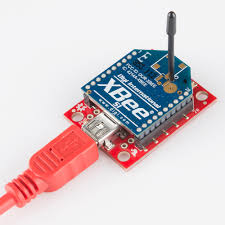
\includegraphics{fig/DOE/XbeeShield}
\caption{Xbee part with Shield}
\end{figure}
In our case, two Ardusat Demosat should send the real time data to the computers seperately.The two XBee parts on Ardusat A and Ardusat B and two Xbee parts pluged in shields are connected to Computers should be set carefully.

\begin{table}[h!]
\renewcommand\arraystretch{2}
	\begin{center}
	\caption{Xbee parts setting}
	\begin{tabular}{|c|c|c|c|c|}
	\hline
	\textbf{Xbee part} & \textbf{A shield} & \textbf{On Ardusat A} & \textbf{B shield} & \textbf{On ArduSat B}\\ \hline
	Channel & \multicolumn{2}{c|}{C} &\multicolumn{2}{c|}{17}  \\ \hline
	Pan ID & \multicolumn{2}{c|}{3332}& \multicolumn{2}{c|}{83D5}\\ \hline
	Destination Address High & 0 & 0 & 0 & 13A200\\ \hline
	Destination Address Low & 35 & 0 & 1234&4163E25D\\ \hline
	16-bit Source Address & 0 & 35 & 4321 & 1532\\ \hline
	Interface Data Rate	 & \multicolumn{4}{c|}{57600}\\ \hline
	Serial Number High & \multicolumn{4}{c|}{13A200}\\ \hline
	Serial Number Low & 4167BD1E & 4163E2BA & 4163E25D & 4167BD2E\\ \hline
	\end{tabular}	
	\end{center}
\end{table}


\newpage